\documentclass{article}
\usepackage[utf8]{inputenc}
\usepackage{graphicx}
\usepackage{subfigure}
\usepackage{listings}
\usepackage{color}
\usepackage{booktabs}
\usepackage{amsmath}
\newcommand{\tabincell}[2]{\begin{tabular}{@{}#1@{}}#2\end{tabular}}
\definecolor{dkgreen}{rgb}{0,0.6,0}
\definecolor{gray}{rgb}{0.5,0.5,0.5}
\definecolor{mauve}{rgb}{0.58,0,0.82}
\lstdefinestyle{myMatlab}{
	frame=l,
	language=Matlab,
	aboveskip=3mm,
	belowskip=3mm,
	showstringspaces=false,
	columns=flexible,
	numberstyle=\small\color{red},
	basicstyle={\small\ttfamily},
	keywordstyle=\color{blue},
	commentstyle=\color{dkgreen},
	stringstyle=\color{mauve},
	breaklines=true,
	breakatwhitespace=true,
	tabsize=3
}

\title{report}
\author{none }
\date{March 2021}

\begin{document}

\maketitle

\section{Data description}
\lstinputlisting[style=myMatlab]{code/nb_industry.m}
Size of data:$[   24934      \quad    49]$.
\\The first column is timestamp that from 1926-07-01 to 2021-02-26.
As the data is a time series and the length of every data is different, the euclidean distance is no longer suitable for the task. The Dynamic Time Warping(DTW) is common used method to dealing with time series data. In the following  will use DTW as the default metric.
\section{Visualization}
We first calculate the pair-wised DTW distances for all samples. And using MDS to visualize the data.

\begin{figure}[!h]
\centering
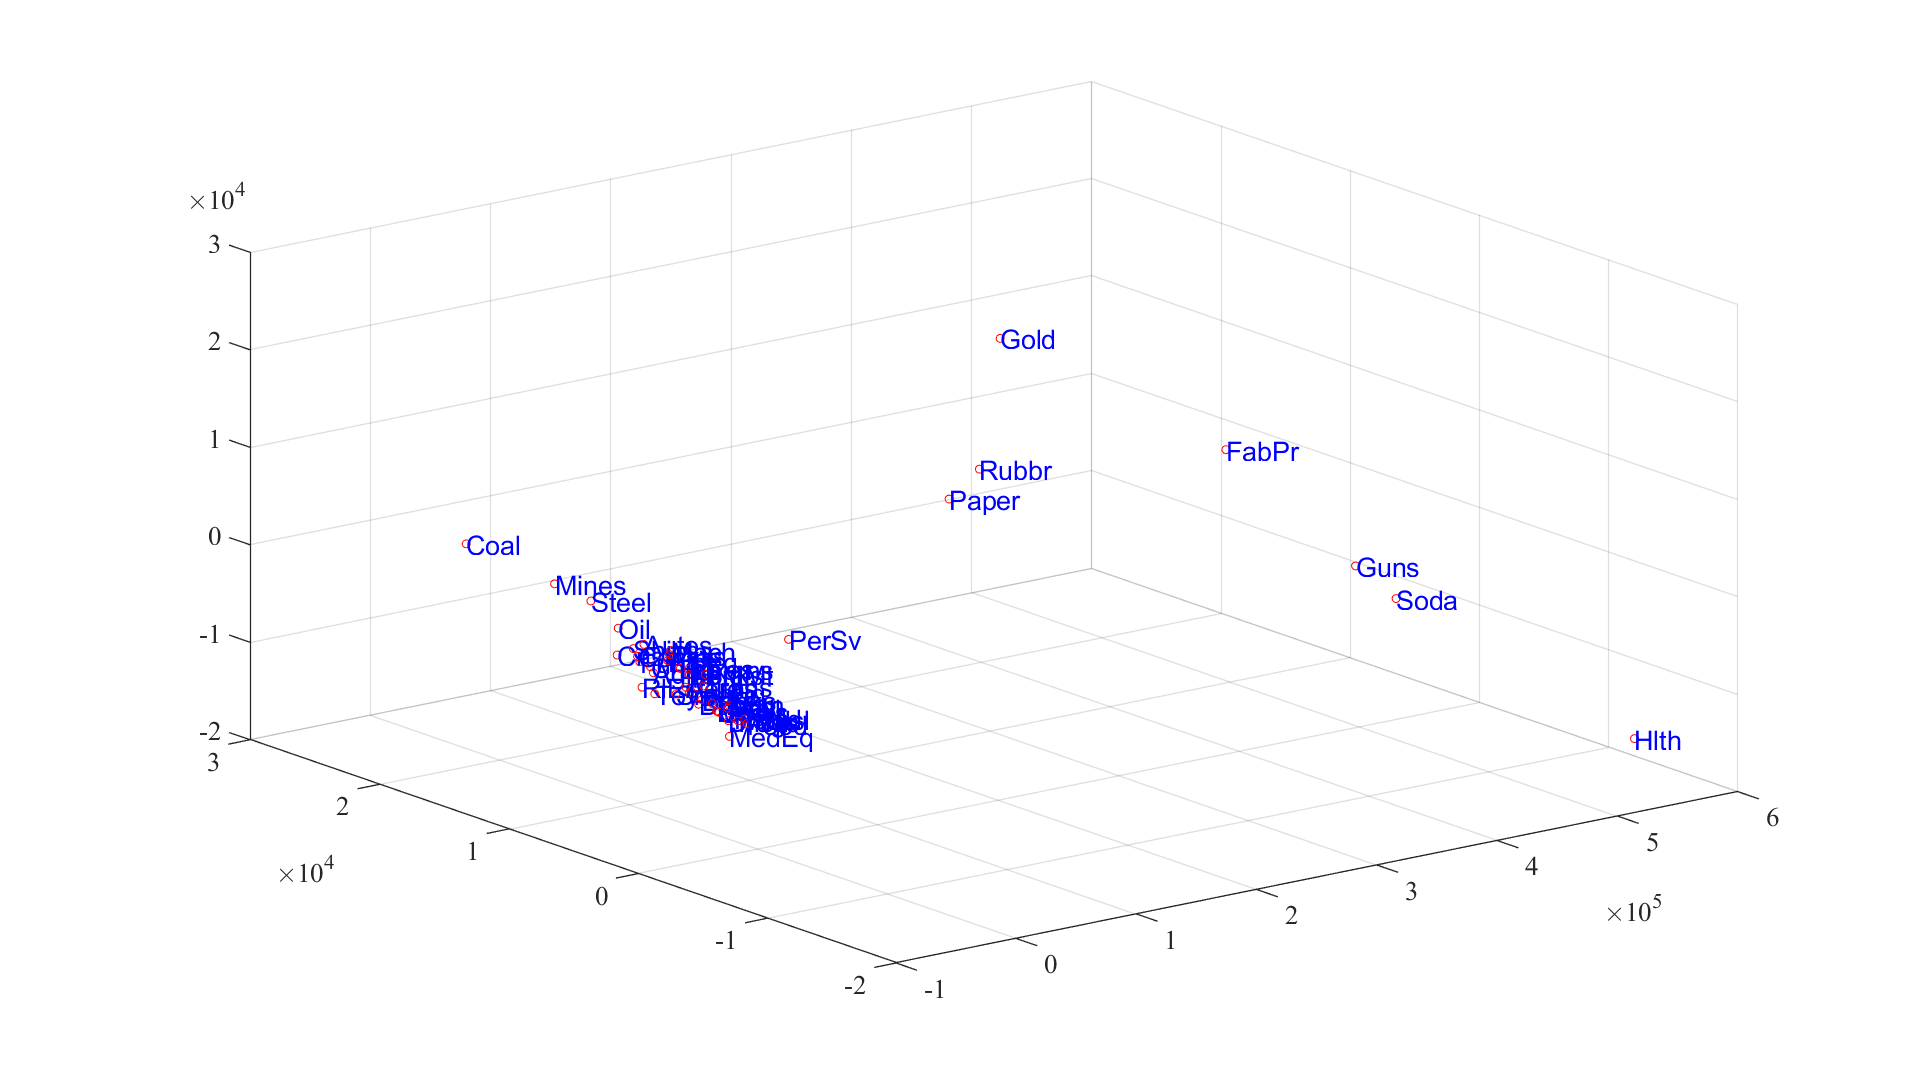
\includegraphics[scale=0.23]{code/original_MDS.png}
\caption{MDS for data}
\label{fig:or_MDS}
\end{figure}
The result reveals that the Gold,Guns,.etc are outline to many samples. They may belong to a same group.


\section{Group cluster}
Then we using hierarchical cluster algorithm to get the hierarchical tree for the DTW dissimilarity matrix.   
\begin{figure}[!h]
\centering
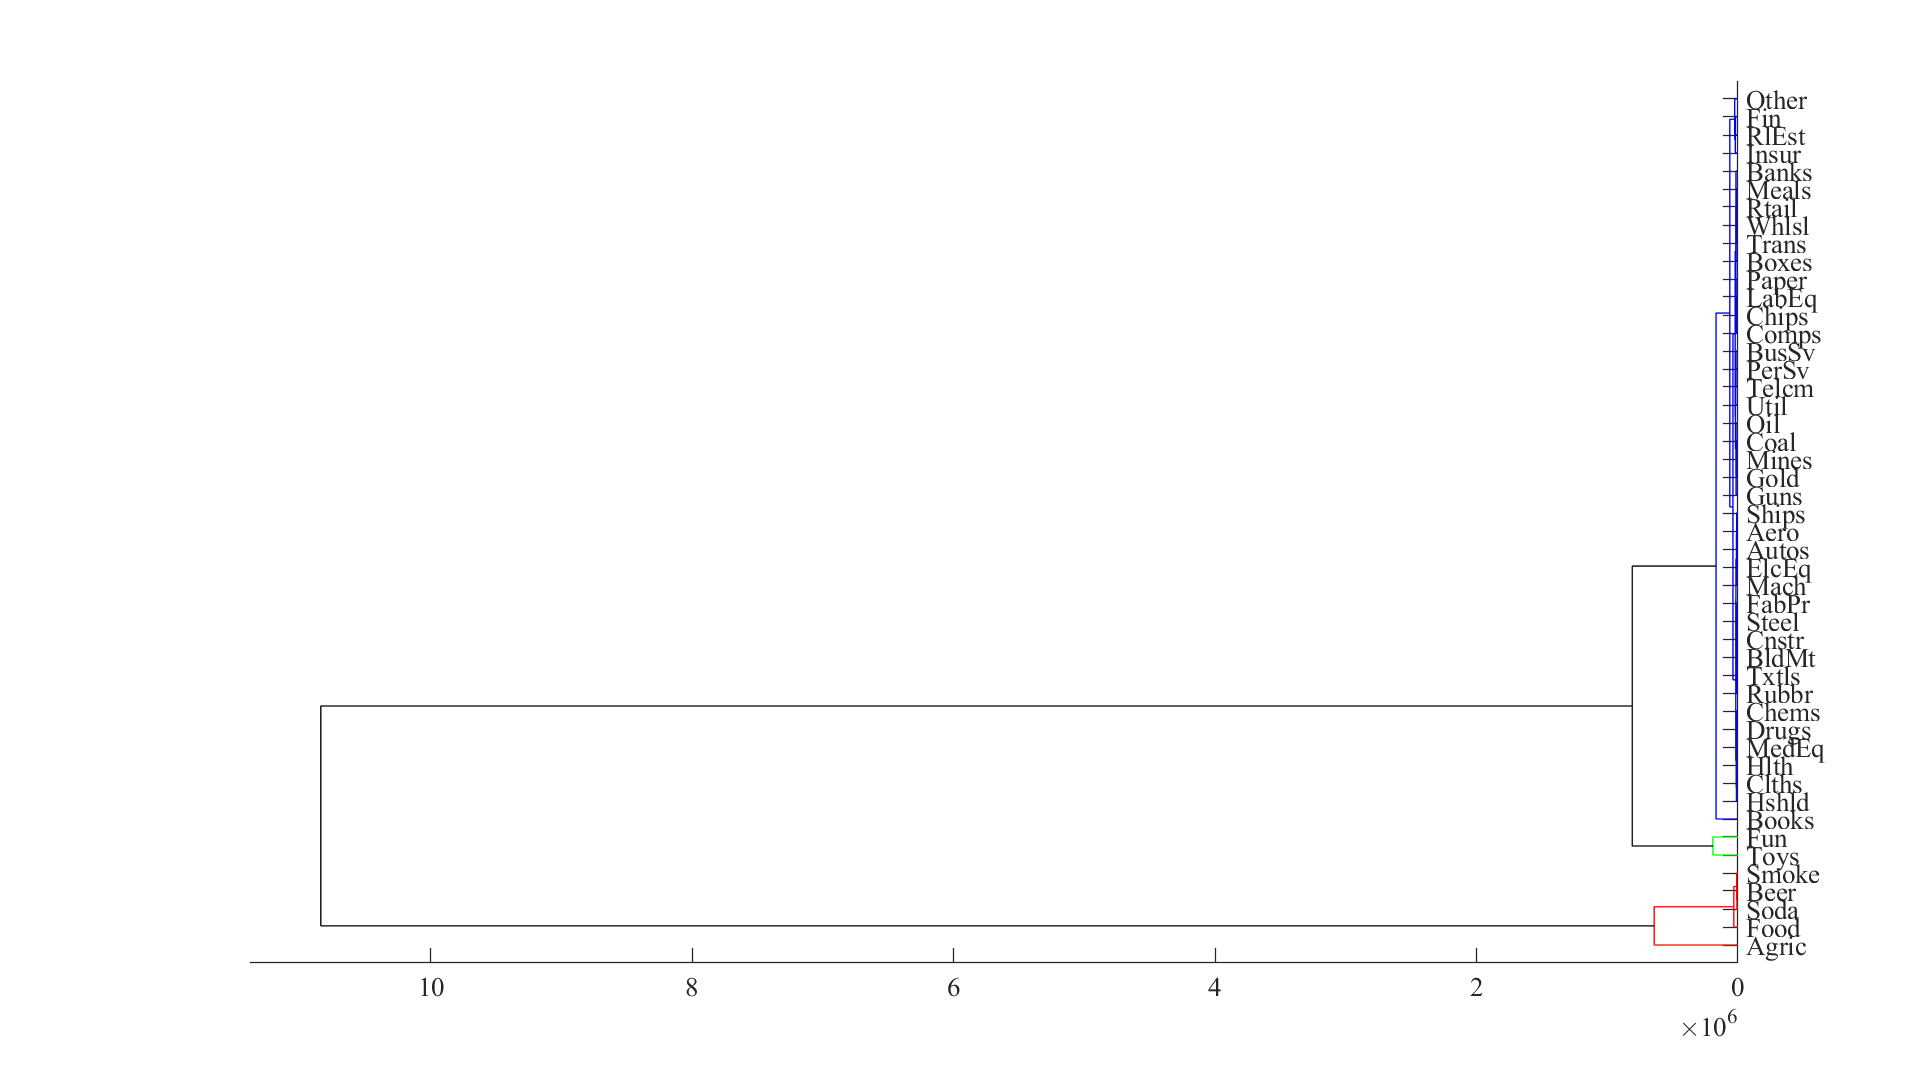
\includegraphics[scale=0.21]{code/original_hi_tree.png}
\caption{Hierarchical tree of data}
\label{fig:or_hitree}
\end{figure}
As the Hierarchical tree far more imbalanced, we weighted the Hierarchical tree.
\begin{figure}[!h]
\centering
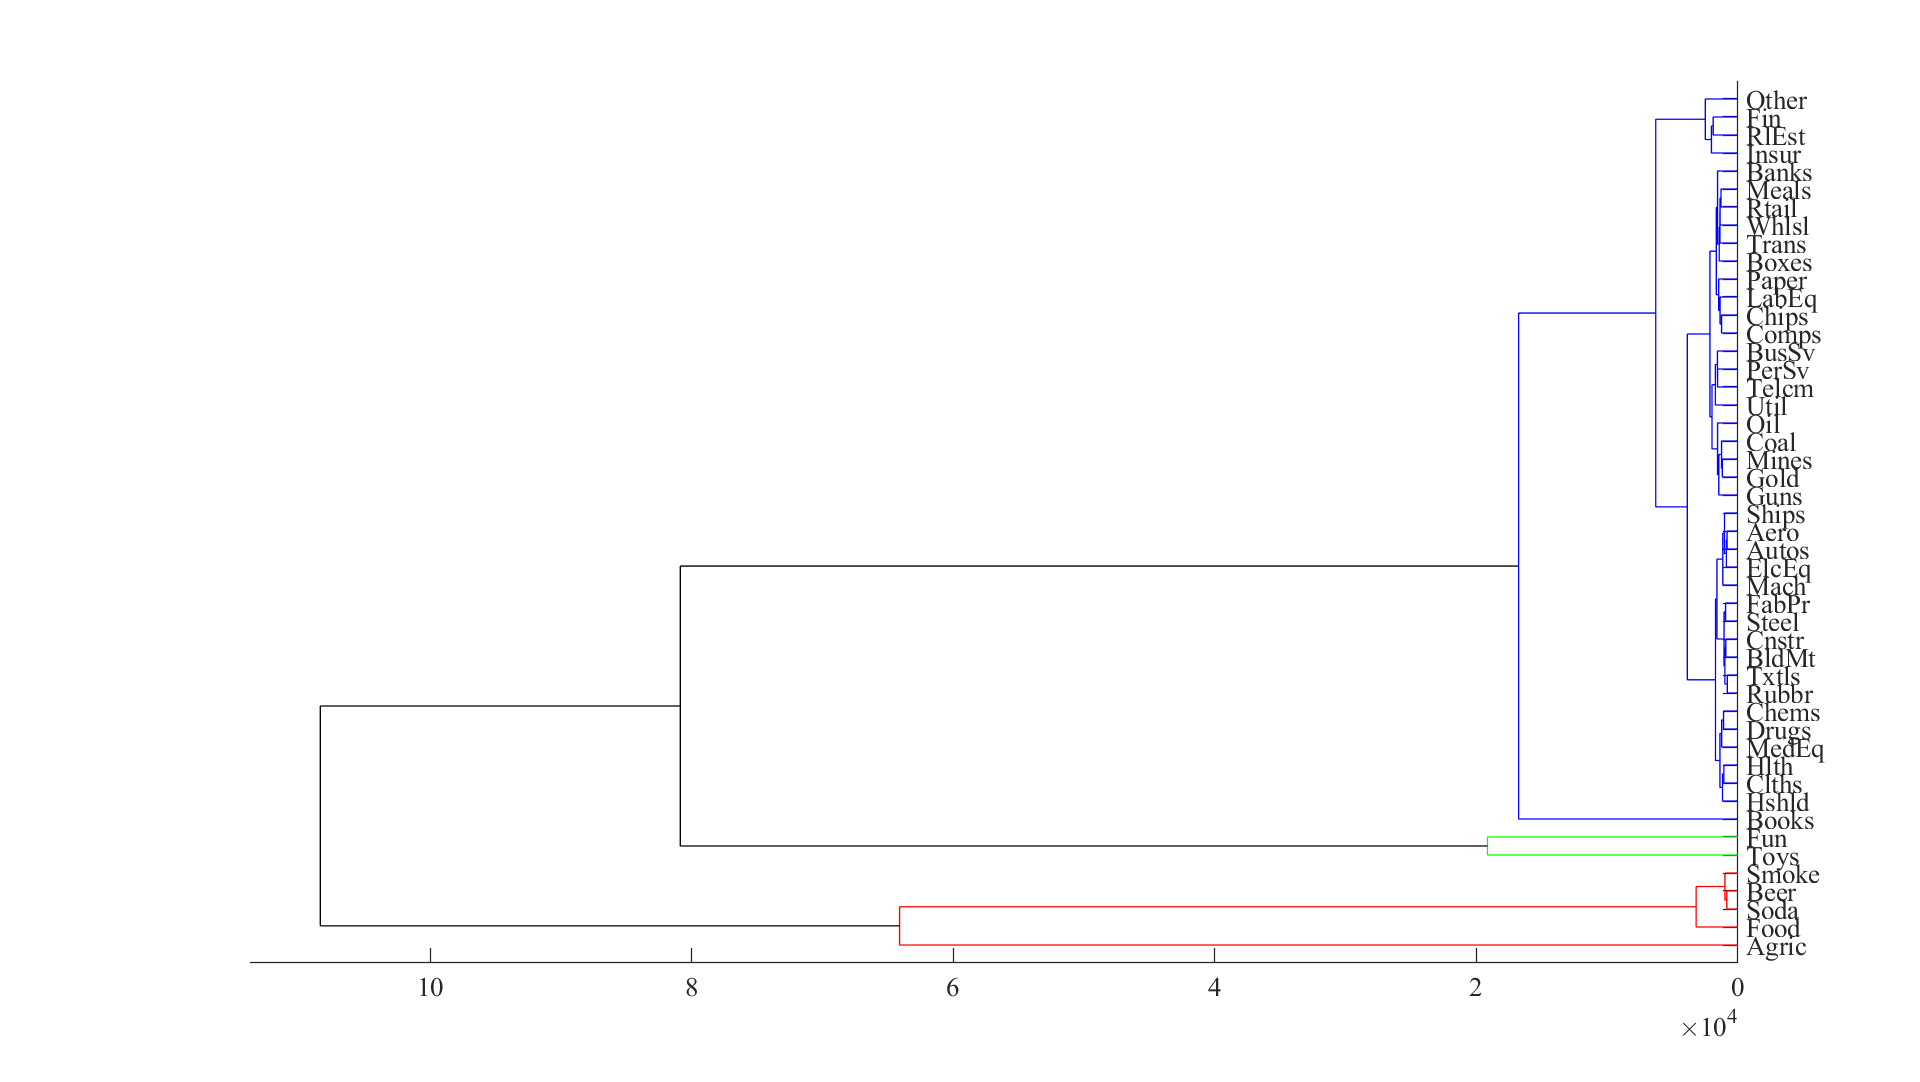
\includegraphics[scale=0.21]{code/hi_tree.png}
\caption{Weighted hierarchical tree of data}
\label{fig:weighted_hitree}
\end{figure}
Showing from the Hierarchical tree, fun and toy are under same tree node, and toy is strong related to fun.
Soda and Beer are under same node which are related in really life, Smoke and food are also relate to these two leaf node. 

Then we construct clusters from this hierarchical cluster tree. 
\begin{figure}[!h]
\centering
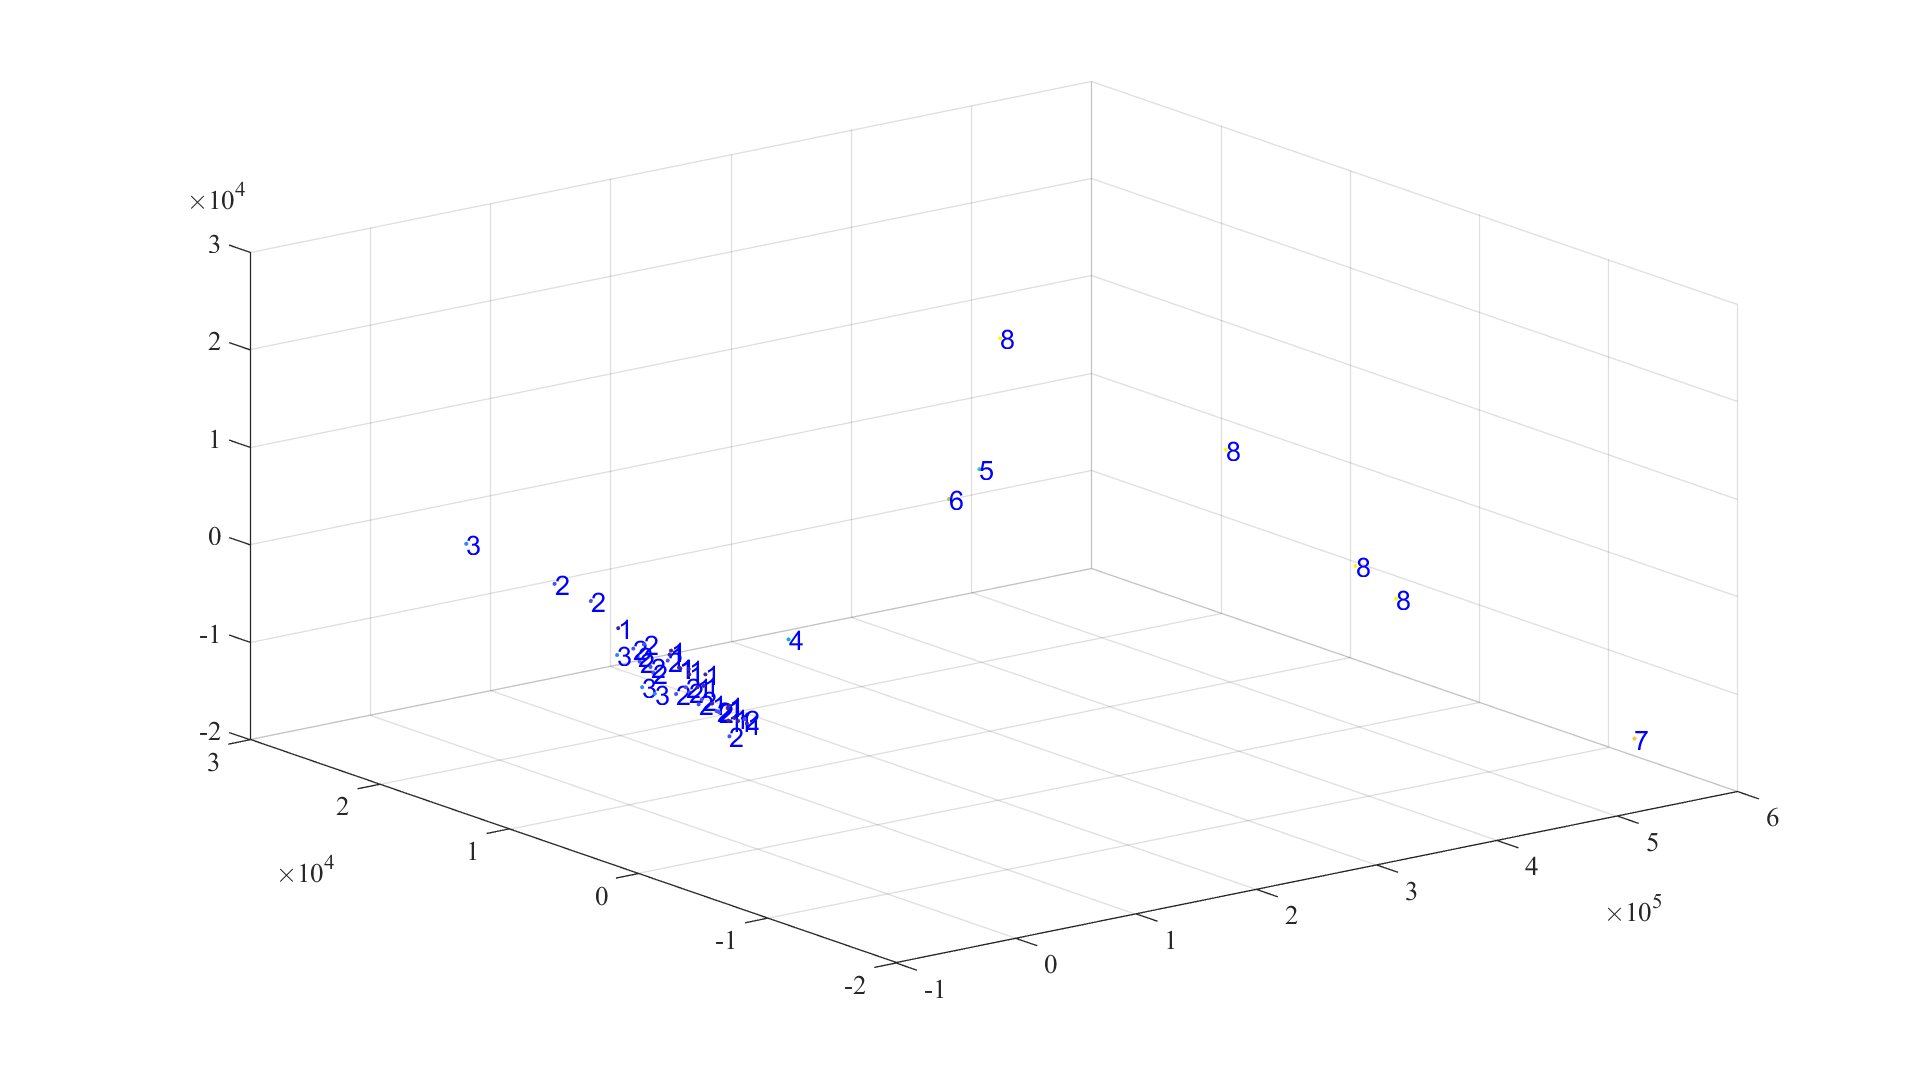
\includegraphics[scale=0.21]{code/8cluster_mds.png}
\caption{Cluster of data}
\label{fig:cluster}
\end{figure}


\begin{table}[h]
\centering
\caption{ cluster information}\label{tab:Rie_sys_kmeans}
\begin{tabular}{|c|c|c|}\hline
%{p{1.4cm}<{\centering}   p{1.4cm}<{\centering}p{1.4cm}<{\centering}}\hline

	cluster&Industry name&number \\\hline
 1&\tabincell{c}{Food,Hshld,Clths,Drugs,Chems,Txtls,BldMt,Mach,\\Oil,Util,Telcm,Boxes,Trans,Rtail,Banks,Insur,Fin}&17 \\\hline
 2&\tabincell{c}{Agric,Beer,Smoke,Fun,Books,MedEq,Steel,ElcEq,Autos,Aero,\\Ships,Mines,BusSv,Comps,Chips,LabEq,Whlsl,Meals,Other}&19 \\\hline
3&\tabincell{c}{Toys,Cnstr,Coal,RlEst}&4 \\\hline
4&PerSv&1 \\\hline
5&Rubbr&1 \\\hline
6&Paper&1 \\\hline
7&Hlth&1 \\\hline
8&\tabincell{c}{Soda,FabPr,Guns,Gold}&4 \\\hline
\end{tabular}

\end{table}
From the plot, we can easily to find out that Guns and Gold belong to same group.

The dissimilar matrix is $X$, $Y(i,j)$ define as follow:

\begin{align*}
\begin{split}
Y(i,j)= \left \{
\begin{array}{ll}
    0,                    & if \quad objects\quad  i\quad  and \quad objects \quad j \quad have\quad  the\quad  same \quad cluster\quad  label\\
    1,     & if \quad not\\
\end{array}
\right.
\end{split}
\end{align*}
To verify whether the 8 is acceptable for the number of cluster, we using $\Gamma$ to verify.
$$\Gamma=\sum^{n-1}_{i=1}\sum^{n}_{j=i+1}X(i,j)*Y(i,j)$$
The $\Gamma=1.278364920250037e+08$. This happened 0.0000999\% for 1000000 random sampled.
The result Higher than 90\% for 1000000 random sampled. Accecpt the number of clusters.
\end{document}
